\documentclass[12pt]{article}
\usepackage{geometry} 
\usepackage{hyperref}
\usepackage{color}
\usepackage[pdftex]{graphicx}  
%\usepackage{caption}
\usepackage{natbib}
\usepackage{authblk}
\usepackage{subscript}
\renewcommand{\baselinestretch}{1.5}
\bibliographystyle{apalike}

\newcommand{\jri}[1]{\textcolor{blue}{ \emph{\scriptsize  #1}} }
\newcommand{\mbh}[1]{\textcolor{red}{ \emph{\scriptsize  #1}} }

%----------------------------------------
%AUTHORS
%----------------------------------------
\title{Natural variation in teosinte at the domestication locus teosinte branched1 (tb1)}

\author[1]{Laura Vann}
\author[1]{Thomas Kono}
\author[1]{Tanja Pyh\"aj\"arvi}
\author[1]{Matthew B. Hufford}
\author[1,2]{Jeffrey Ross-Ibarra\thanks{rossibarra@ucdavis.edu}}
\affil[1]{Department of Plant Sciences, University of California Davis}
\affil[2]{Center for Population Biology and Genome Center, University of California Davis}

\begin{document}

\maketitle

\jri{Please add addresses for all authors.  All should have plant sciences, but Kono, Tanja, and Huff need their new addresses too. }

\mbh{my new address is: Department of Ecology, Evolution, and Organismal Biology, Iowa State University, Ames, IA, 50011}

\clearpage

\subsection*{Abstract}

The \emph{teosinte branched1} (\emph{tb1}) gene, a repressor of lateral organ growth, is a major QTL involved in branching differences between maize and its wild progenitor, teosinte. Further studies have shown that the insertion of a transposable element (Hopscotch) upstream of tb1 enhances its expression, causing the reduction in branching observed in domesticated maize. Observations of the maize \emph{tb1} allele in teosinte individuals, coupled with estimates of the age of insertion of the Hopscotch element, led us to investigate the role of \emph{tb1} in teosinte. Results from genotyping across many natural populations suggest that the Hopscotch element is segregating at a higher than expected frequency in a number of populations of both subspecies \emph{parviglumis} and \emph{mexicana}. Analysis of linkage disequilibrium between the Hopscotch element and variation in surrounding regions does not support a hypothesis of recent introgression from maize into teosinte, and we find no evidence of environmental correlations that might suggest recent selection.  Finally, two greenhouse experiments fail to find an important role for \emph{tb1} in controlling tillering in natural populations of \emph{parvilgumis}. \jri{Needs a concluding sentence. "Thus, we think..." or something.} 

\clearpage

\section*{Introduction}

Domesticated crops and their wild progenitors provide an excellent system in which to study adaptation and genomic changes associated with human-mediated selection \cite{Ross-Ibarra et al 2007}. Perhaps the central focus of the study of domestication has been the identification of genetic variation underlying agronomically important traits such as fruit size and plant architecture \cite{OlsenGross2010}. \jri{I believe you need to remove spaces from the bibtex citation names.  See how this OlsenGross2010 works but the others don't? should be able to work with whitespace but i can't figure out why not.}  Additionally, many domesticates show reduced genetic diversity when compared to their wild progenitors, and an understanding of the distribution of diversity in the wild and its phenotypic effects has become increasingly useful to crop improvement \cite{Kovach and McCouch 2008}. But while some effort has been invested into understanding how wild alleles behave in their domesticated relatives, very little is known about the role that alleles found most commonly in domesticates play in natural populations of their wild progenitors.

% SFS figure
%-------------------------------------------------------------------
\begin{figure*}[!t]
  \begin{center}
   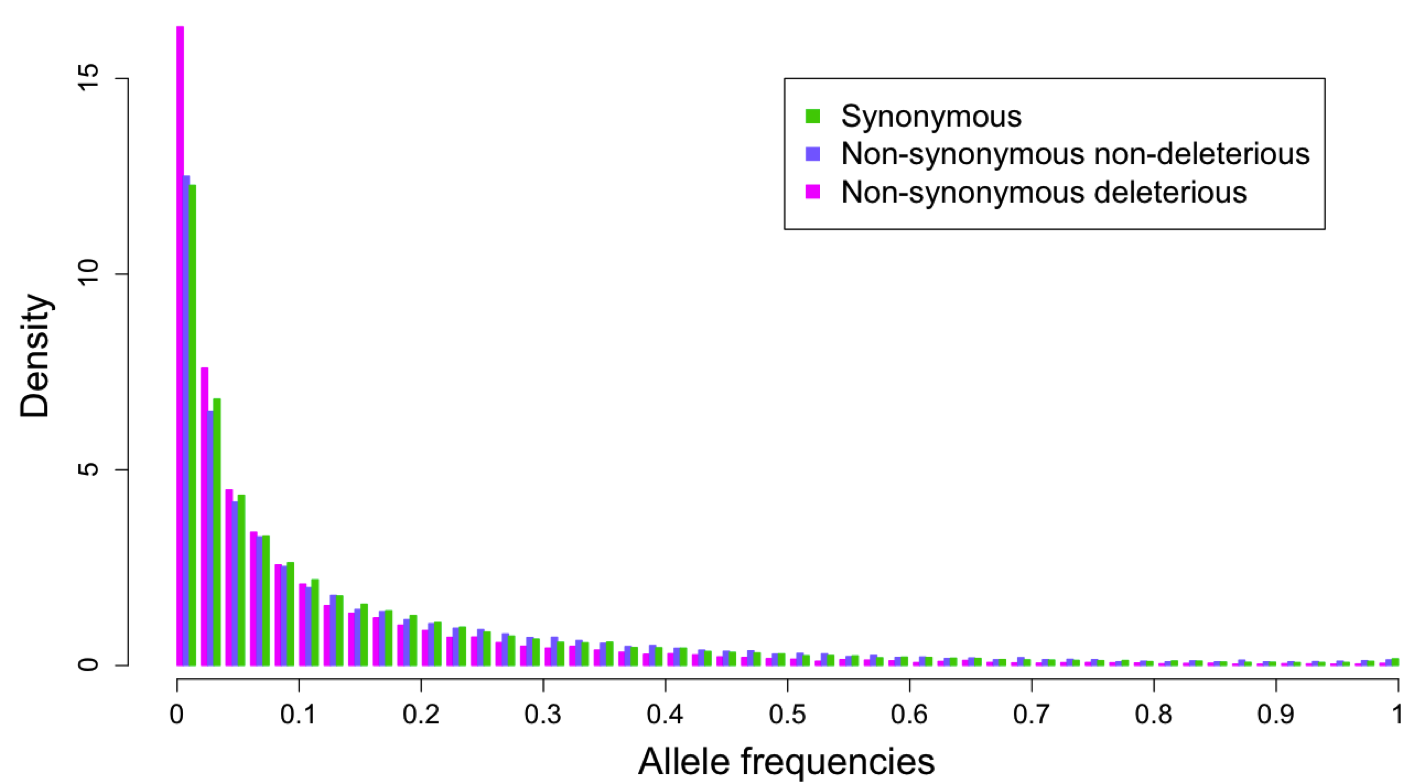
\includegraphics[width=150mm]{SFS.png}
    \caption{This is an example figure.} 
\label{sfs_non_syn}
  \end{center}
\end{figure*}
%-------------------------------------------------------------------

\jri{This is how you cite the figure in the text. "I want to show you all Figure \ref{sfs_non_syn}." Latex takes care of the numbering.  Please add all the figures to the text, and add them in in the middle like this close to where they are referenced. Note that it puts the figure where it thinks best, which is not necessarily near this text.}

Maize (\emph{Zea mays} ssp. \emph{mays}) was domesticated from the teosinte \emph{Zea mays} ssp. \emph{parviglumis} (hereafter, \emph{parviglumis}) roughly 10,000 B.P. in southwest Mexico \cite{Piperno et al 2009, Matsuoka et al 2002}. Domesticated maize and the teosintes are an attractive system in which to study domestication due to the abundance of genetic tools developed for maize and well-characterized domestication loci \cite{Hufford et al 2012a, Doebley 2004, Hufford et al 2012b}. Additionally, large naturally occurring populations of both \emph{Zea mays} ssp. \emph{parviglumis} (the wild progenitor of maize) and \emph{Zea mays} ssp. \emph{mexicana} (highland teosinte) can be found throughout Mexico \cite{Wilkes 1977, Hufford et al 2013}, and genetic diversity and effective population size (Ne) of these taxa is estimated to be high \cite{Ross-Ibarra et al 2009} relative to other plants \cite{Nybom 2004}.

Many morphological changes are associated with the domestication of maize, and understanding the genetic basis for these changes has been a focus of maize research for a number of years. One of the most dramatic changes is found in plant architecture: domesticated maize is characterized by a central stalk with few tillers and lateral branches terminating in a female inflorescence, while teosinte is highly tillered and bears tassels (male inflorescences) at the end of its lateral branches. The \emph{teosinte branched1} (\emph{tb1}) gene, a repressor of organ growth, was identified as a major QTL involved in branching differences between maize and teosinte \cite{Doebley et al 1990, Doebley and Stec 1991, Lukens and Doebley 1999}. Further studies have shown that the insertion of a 4.9 kb retrotransposon (Hopscotch) in the upstream control region of \emph{tb1} led to increased expression of this gene, causing the reduction in branching observed in domesticated maize \cite{Studer et al 2011}. The effects of this insertion have been observed in tiller number in maize, but little is known about its role, if any, in teosinte \cite{Studer et al 2011}. Dating of this element has suggested that its insertion predates the domestication of maize, leading to the hypothesis that it was segregating as standing variation in ancient populations of teosinte and increased to high frequency in maize due to selection during domestication \cite{Studer et al 2011}. Furthermore, \cite{Studer and Doebley 2012} investigated the phenotypic effects of 9 teosinte \emph{tb1} alleles in an isogenic maize background and found that the introgressions sort into three distinct phenotypic classes, suggesting that variation at the \emph{tb1} locus may play a functional role in teosinte. \mbh{A sentence or two is needed here explaining why tillering may be an ecologically relevant trait to a wild plant} In this study we aim to characterize the distribution of the Hopscotch insertion in \emph{mexicana}, \emph{parviglumis}, and landrace maize, and to examine the phenotypic effects of the insertion in \emph{parviglumis}. We use a combination of PCR genotyping for the Hopscotch element in our full panel and sequencing of two small regions upstream of \emph{tb1} in a subset of teosinte populations to explore patterns of genetic variation at this locus. Finally, we test for an association between the Hopscotch element and tillering phenotypes in a population of \emph{parviglumis}.

 
\section*{Methods}

\subsection*{Sampling and Genotyping}

We sampled 1,110 individuals from 350 accessions (247 maize landraces, 17 Zea mays ssp. mexicana (hereafter mexicana) populations, and 86 \emph{parviglumis} populations) and assessed the presence or absence of the Hopscotch insertion (Table S1, Table S2). \jri{please add tables and reference same as figs; see example in Sofiane's "deleterious 282" repo on lab github page} DNA was extracted from leaf tissue using a modified CTAB approach \cite{Doyle and Doyle 1990, Maloof et al 1984}. We designed primers using PRIMER3 \cite{Rozen and Skaletsky 2000} implemented in Geneious \cite{Kearse et al 2012} to amplify the entire Hopscotch element, as well as an internal primer allowing us to simultaneously check for possible PCR bias between presence (~5 kb amplification product) and absence (~300 bp amplification product) of the Hopscotch insertion. Two PCRs were performed for each individual, one with primers flanking the Hopscotch (HopF/HopR) and one with a flanking primer and an internal primer (HopF/HopIntR). Primer sequences are HopF, 5'-TCGTTGATGCTTTGATGGATGG-3'; 
Hop R, 5'-AACAGTATGATTTCATGGGACCG-3'; and HopIntR, 5'-CCTCCACCTCTCATGAGATCC-3' (Figure S1). \jri{supplemental material should be added to this file too.} Homozygotes show a single band for either the Hopscotch element (~5 kb) or the absence of the element (~300 bp), while heterozygotes are three-banded, showing a band for both the presence and absence of the Hopscotch element as well as a band for the internal primer set (Figure S2). When only one PCR resolved well, we scored one allele for the individual, which explains the odd number of alleles included in our analyses. We used Phusion High Fidelity Enzyme (Finnzymes, Inc.) and the following conditions for amplifications: 98°C for 3 min, 30 cycles of 98°C for 15 s, 65°C for 30 s, and 72°C for 3 min 30 s, with a final extension of 72°C for 10 min. PCR products were visualized on a 1\% agarose gel and scored for presence/absence of the Hopscotch based on band size.

\subsection*{Sequencing}

In addition to genotyping, we chose a subset of \emph{parviglumis} individuals for sequencing. We chose twelve individuals from each of four populations from Jalisco state, Mexico (San Lorenzo, La Mesa, Ejutla A, and Ejutla B). For amplification and sequencing, we selected two regions approximately 600bp in size from within the 5' UTR of \emph{tb1} (sequenced region 1) and from 1,235 bp upstream of the start of the Hopscotch and 66,169 bp upstream from the start of the \emph{tb1} ORF (sequenced region 2). The 5' UTR (containing sequenced region 1) has been shown to have elevated diversity in ssp. \emph{parviglumis} with respect to maize, while the the area upstream from the Hopscotch (sequenced region 2) has been shown to be critical in determining basal branching and ear architecture \cite{Wang et al 1999, Clark et al 2006}. We designed the following primers using PRIMER3 \cite{Rozen and Skaletsky 2000}: for the 5' UTR, 5' GGATAATGTGCACCAGGTGT 3' and 5' GCGTGCTAGAGACACYTGTTGCT 3'; for the 50 kb upstream region, 5' TGTCCTCGCCGCAACTC 3' and 5' TGTACGCCCGCCCCTCATCA 3' (Figure S1). We used Taq Polymerase (New England Biolabs) and the following thermal cycler conditions to amplify fragments: 94°C for 3 min, 30 cycles of 92°C for 40 s, annealing for 1 min, 72°C for 40 s, and a final 10 min extension at 72°C. Annealing temperatures for sequenced region 1 and sequenced region 2 were 59.7°C and 58.8°C, respectively. To clean excess primer and dNTPs we added two units of Exonuclease1 and 2.5 units of Antarctic Phosphatase to 8.0 µL of amplification product. This mix was placed on a thermal cycler with the following program: 37°C for 30 min, 80°C for 15 min, and a final cool-down step to 4°C. 

We cloned cleaned fragments into a TOPO-TA vector (Invitrogen, Carlsbad) using OneShot TOP10 chemically competent E. coli cells, with an extended ligation time of 30 min for a complex target fragment. We plated cells on LB agar plates containing kanamycin, and screened colonies using vector primers M13 Forward and M13 Reverse under the following conditions: 96°C for 5 min; then 35 cycles at 96°C for 30 s, 53°C for 30 s, 72°C for two min; and a final extension at 72°C for 4 min. We visualized amplification products for incorporation of our insert on a 1\% agarose TAE gel.

Amplification products with successful incorporation of our insert were cleaned using Exonuclease 1 and Antarctic Phosphatase following the procedures detailed above, and sequenced with vector primers M13 Forward and M13 Reverse using Sanger sequencing at the College of Agriculture and Environmental Sciences (CAES) sequencing center at UC Davis. We aligned and trimmed primer sequences from resulting sequences using the software Geneious \cite{Kearse et al 2012}. Following alignment, we verified singleton SNPs by sequencing an additional one to four colonies from each clone. If the singleton was not present in these additional sequences it was considered an amplification or cloning error, and we replaced the base with the base of the additional sequences. If the singleton appeared in at least one of the additional sequences we considered it a real variant and kept it for further analyses. 

\subsection*{Genotyping Analysis}

We examined discrepancies between observed and expected genotype frequencies by calculating Hardy-Weinberg Equilibrium (HWE), and to calculate differentiation between populations (F\textsubscript{ST}) and subspecies (F\textsubscript{CT}) we used HierFstat \cite{Goudet 2005}. These analyses only included populations in which 8 or more individuals were sampled. To test the hypothesis that the Hopscotch insertion may be adaptive under certain environmental conditions, we looked for significant associations between the Hopscotch frequency and environmental variables using BayEnv \cite{Coop et al 2010}. BayEnv creates a covariance matrix of relatedness between populations, and then tests a null model that allele frequencies in populations are determined by the covariance matrix of relatedness alone against the alternative model that allele frequencies are determined by a combination of the covariance matrix and an environmental variable, producing a posterior probability (Bayes Factor)\cite{Coop et al 2010}. We used genotyping and covariance data from Pyhäjärvi et al., (2013) \cite{Pyhajarvi et al 2013} for BayEnv, with the Hopscotch insertion coded as an additional SNP (Table S3). Environmental data were obtained from www.worldclim.org, the Harmonized World Soil Database and www.harvestchoice.org, and summarized by principle component analysis Pyhäjärvi et al. (2013) \cite{Pyhajarvi et al 2013}.

\subsection*{Sequence Analysis}

For population genetic analyses of sequenced region 1 and sequenced region 2 we used the analysis package of Libsequence \cite{Thornton 2003} to calculate pairwise F\textsubscript{ST} between populations, and to calculate standard diversity statistics (number of haplotypes; haplotype diversity; Watterson's estimator $\theta_{W}$; pairwise nucleotide diversity $\theta_{\pi}$; and Tajima's D). To produce a visual representation of differentiation between sequences and to examine patterns in sequence clustering by Hopscotch genotype we used Phylip (http://evolution.genetics.washington.edu/phylip.html) to create neighbor-joining trees with bootstrapping (100 repetitions) to examine the support of nodes in our trees. For creation of trees we also included homologous sequence data from teosinte inbred lines (TILs), some of which are known to be homozygous for the Hopscotch insertion (TIL03, TIL17, TIL09), as well as 59 lines of domesticated maize and landraces (data from Maize HapMapV2, \cite{Chia et al 2012}).

In order to assess patterns of linkage disequilibrium (LD) around the Hopscotch element in the context of chromosomal patterns of LD we used Tassel \cite{Bradbury et al 2007} and calculated LD between SNPs across chromosome 1 using previously published data from twelve plants each of the Ejutla A, Ejutla B, San Lorenzo, and La Mesa populations \cite{Pyhajarvi et al 2013}. We chose these populations because we had both genotyping data for the Hopscotch as well as chromosome-wide SNP data for chromosome 1. For each population we filtered the initial set of 5,897 SNPs on chromosome 1 to accept only SNPs with a minor allele frequency of at least 0.1, resulting in 1,671, 3,023, 3,122, and 2,167 SNPs for San Lorenzo, Ejutla B, Ejutla A, and La Mesa, respectively. We then used Tassel \cite{Bradbury et al 2007} to calculate linkage disequilibrium ($r^{2}$) across chromosome 1 for each population. 

We examined evidence of introgression on chromosome 1 in these same four populations (EjuA, EjuB, MSA, SLO) using STRUCTURE \cite{Falush et al 2003} and the same phased 55K SNP data from \cite{Pyhajarvi et al 2013} that we used for LD analysis, combined with the corresponding SNP data from a diverse panel of 282 maize lines \cite{Cook et al 2012}. SNPs were anchored in a modified version of the IBM genetic map ( \cite{Gerke et al 2013}, \url{http://arxiv.org/abs/1307.7313}). We created haplotype blocks using a custom Perl script that grouped SNPs separated by less than 5kb into haplotypes. We ran STRUCTURE at K=2 under the linkage model, performing 3 replicates with an MCMC burn-in of 10,000 steps and 50,000 steps post burn-in. 

\subsection*{Phenotyping of \emph{Zea mays.} ssp. \emph{parviglumis}}

To investigate the phenotypic effects of the Hopscotch insertion in teosinte, we conducted an initial phenotyping trial (Phenotyping 1). We germinated 250 seeds of \emph{parviglumis} collected in Jalisco state, Mexico (population San Lorenzo) \cite{Hufford 2010} where the Hopscotch is segregating at highest frequency (0.4375) in our initial genotyping sample set. In order to maximize the likelihood of finding the Hopscotch in our association population we selected seeds from sites where genotyped individuals were homozygous or heterozygous for the insertion. We chose between 10-13 seeds from each of 23 sampling sites. We treated seeds with fungicide and germinated them in petri dishes with filter paper. Successful germinations (206 individuals) were then planted into one gallon size pots with potting soil and randomly spaced one foot apart on greenhouse benches. Plants were watered three times a day with an automatic drip containing 10-20-10 fertilizer. 

Starting on day 15, we measured tillering index, the ratio of the sum of tiller lengths to the height of the plant \cite{Briggs et al 2007}. Tillering index has been shown to be the most effective way to observe the phenotypic effects of the Hopscotch insertion on plant architecture in maize \cite{Briggs et al 2007}. Following initial measurements, we phenotyped plants for tillering index every 5 days through day 40, and then on day 50 and day 60. On day 65 we measured culm diameter between the third and fourth nodes of each plant. Culm diameter is not believed to be correlated with tillering index, or variation at \emph{tb1} (e.g. Hopscotch genotype). Following phenotyping we extracted DNA from all plants using a modified SDS extraction protocol (http://www.ars.usda.gov). We genotyped individuals for the Hopscotch insertion following the protocols listed above. Based on these initial data, we conducted a post hoc power analysis using data from day 40 of phenotyping 1, indicating that a minimum of 71 individuals in each genotype class are needed to detect the observed effect of the Hopscotch on tillering index.

We performed a second phenotyping experiment (phenotyping 2) in which we germinated 372 seeds of \emph{parviglumis}, choosing equally between sites previously determined to have or not have the Hopscotch insertion. Seeds were germinated and planted on day 7 post fruit-case removal into 2 gallon pots. Plants were watered twice daily, alternating between fertilized and non-fertilized water. We began phenotyping successful germinations (302) for tillering index on day 15 post fruit case removal, and phenotyped every five days until day 50. At day 50 we measured culm diameter between the third and fourth nodes. We extracted DNA and genotyped plants following the same guidelines as in phenotyping 1. 

Resulting tillering index data for each genotype class did not meet the criteria for a repeated measures ANOVA, so we transformed the data using a Box-Cox transformation ($\alpha=0$) implemented in the car package in R \cite{Fox and Weisberg 2011} to improve the normality and homogeneity of variance among genotype classes.  We analyzed relationships between genotype and tillering index and tiller number using a repeated measures ANOVA through a general linear model function implemented in SAS v.9.3 (SAS Institute Inc., Cary, NC, USA). Additionally, in order to compare any association between Hopscotch genotype and tillering and associations at other presumably unrelated traits, we performed an ANOVA between culm diameter and genotype using the same general linear model in SAS. 

\section*{Results}

\subsection*{Genotyping}

We genotyped 247 accessions of maize landraces, and found the Hopscotch element fixed in all but 8 of these accessions (inbred lines X,Y, Z, and landraces in Chihuahua, Tapalpa, Tenancingo, and Altotonga) (Table S1, Table S2). For all analyses we only included individuals that clearly resolved for both PCRs, resulting in 837 individuals total. Within our \emph{parviglumis} and \emph{mexicana} samples we found the Hopscotch insertion segregating in 37 and 4 populations, respectively, and at highest frequency in the states of Jalisco, Colima, and Michoac\'{a}n in central-western Mexico in both subspecies (Figure 1). We examined Hardy-Weinberg equilibrium in a total of 14 populations (10 \emph{parviglumis} and 4 \emph{mexicana}) with more than 8 individuals sampled per population. Three populations (RIMPA0073, RIMPA0093, and RIMPA0158) show evidence of deviations from expected genotype frequencies under the assumptions of HWE (p=0.05). \mbh{not sure what p=0.05 means here.  Should it be p $<$ 0.05 or $\alpha$ = 0.05?} 

Using our Hopscotch genotyping data, we calculated differentiation between populations (F\textsubscript{ST}) and subspecies (F\textsubscript{CT}) for populations in which we sampled 8 or more alleles. F\textsubscript{CT} is 0 within our dataset, and we found similar levels of F\textsubscript{ST} between populations within each subspecies (0.22) and between all populations (0.23), to those reported in genome-wide estimates from previous studies \cite{Pyhajarvi et al 2013} (Table 1). Although we found large variation in Hopscotch allele frequency among our populations, our BayEnv analysis did not indicate a correlation between the Hopscotch insertion and environmental variables (all Bayes Factors $<$ 1; Table S3). 

\subsection*{Sequencing}

To investigate patterns of sequence diversity and linkage disequilibrium (LD) in the tb1 region, we sequenced two small ($<$1kb) regions upstream of the tb1 ORF in four populations. After alignment and singleton checking we recovered 40 and 48 segregating sites for the 50kb upstream region and the 5' UTR region, respectively. For region 1, Ejutla A, Ejutla B, and La Mesa have comparable values for haplotype diversity, $\theta_{W}$, $\theta_{\pi}$, and Tajima's D, while San Lorenzo has lower values for haplotype diversity, $\theta_{W}$, $\theta_{\pi}$, and a more positive value for Tajima's D (Table 2). For region 2, haplotype diversity, $\theta_{W}$, and $\theta_{\pi}$, are similar for Ejutla A and Ejutla B, while La Mesa and San Lorenzo have slightly lower values for these statistics (Table 2). Tajima's D is positive in all populations except San Lorenzo, indicating an excess of low frequency variants in this latter population (Table 2). \mbh{this text hasn't changed since the last time I read the manuscript and previously did not agree with the results presented in Table 2.  Was Table 2 incorrect?} Pairwise values of F\textsubscript{ST} within population pairs Ejutla A/Ejutla B and San Lorenzo/La Mesa are 0 for both sequenced regions as well as for the Hopscotch, while they are high for other population pairs (Table 1). Neighbor joining trees of our sequence data and data from the teosinte inbred lines (TILS; data from Maize HapMapV2, \cite{Chia et al 2012}) do not reveal any clear clustering pattern with respect to population or Hopscotch genotype (Figure S3). Furthermore, individuals within our sample that have the Hopscotch insertion do not group with the teosinte inbred lines or the lines of domesticated maize that have the Hopscotch insertion. 

\subsection*{Evidence of introgression}

The teosinte populations with the highest frequency of the Hopscotch insertion in this study were sympatric with cultivated maize. Our initial hypothesis was that the high frequency of the Hopscotch element in these populations could be attributed to introgression from maize into teosinte. To investigate this possibility we examined overall patterns of linkage disequilibrium across chromosome one, and specifically in the \emph{tb1} region. If the Hopscotch is found in these populations due to recent introgression we would expect to find large blocks of linked markers near this element. We find no evidence of elevated linkage disequilibrium between the Hopscotch and SNPs surrounding the tb1 region in our resequenced populations (Figure 2), and $r^{2}$ in the \emph{tb1} region (positions 264,596,664-265,891,456; AGPv2) does not differ significantly between populations with (average $r^{2}$ of 0.085) and without the Hopscotch genotype (average $r^{2}=0.082$). In fact, average $r^{2}$ is lower in the \emph{tb1} region ($r^{2}=0.056$) than across the rest of chromosome 1 ($r^{2}=0.083$) (Table 3). 

The lack of clustering of Hopscotch genotypes in our NJ tree as well as the lack of LD around \emph{tb1} does not support the hypothesis that the Hopscotch insertion in these populations of \emph{parviglumis} is the result of recent introgression. However, to further explore this hypothesis we performed a STRUCTURE analysis using Illumina MaizeSNP50 data from four of our \emph{parviglumis} populations (EjuA, EjuB, MSA, and SLO) and the maize 282 diversity panel \cite{Cook et al 2012, Phyhajarvi et al 2013}. The linkage model implemented in STRUCTURE can be used to identify ancestry of blocks of linked variants, which would arise as a result of recent admixture between populations. If the Hopscotch insertion is present in populations of \emph{parviglumis} as a result of recent admixture with domesticated maize, we would expect the insertion and linked variants in surrounding sites to be assigned to the "maize" cluster in our STRUCTURE runs, not the "teosinte" cluster. In all runs, assignment to maize in the \emph{tb1} region across all four \emph{parviglumis} populations is lower (average 0.017) than the chromosome wide average (0.20; Figure 3). 

\subsection*{Phenotyping}

\subsubsection*{Phenotyping 1}

We measured tillering index (TI), the ratio of the sum of tiller lengths to plant height, for 216 plants from 23 sampling locations within the San Lorenzo population, and genotyped plants for the Hopscotch insertion. We found the Hopscotch segregating at a frequency of 0.65; with a 0.4 frequency of homozygotes for the Hopscotch, a 0.5 frequency of heterozygotes, and a 0.1 frequency of homozygotes for the teosinte allele (no Hopscotch), showing no significant deviations from expected frequencies under Hardy-Weinberg equilibrium. After performing a repeated measures ANOVA between our transformed tillering index data and Hopscotch genotype we find a weak positive correlation between presence of the Hopscotch and tillering index on day 40 (p=0.0848), but no correlation between tillering index and genotype on any other day (Figure 4). Additionally we find no significant correlation between tiller number and Hopscotch genotype, or culm diameter and Hopscotch genotype in phenotyping 1.

\subsubsection*{Phenotyping 2}

For phenotyping 2 we measured tillering index every five days through day 50 for 302 plants. We followed the same transformations and analyses as described in phenotyping 1. We find the Hopscotch allele segregating at a frequency of 0.69, with a 0.6 frequency of Hopscotch homozygotes, and a 0.2 frequency of both heterozygotes and homozygotes for the teosinte allele. We find similar patterns as in phenotyping 1, with a weak positive correlation between tillering index and Hopscotch genotype at day 40 (p=0.0611), with no significant correlation on any day. Similarly, relationships between Hopscotch genotype and tiller number, and hopscotch genotype and culm diameter are not significant. 


\section*{Discussion}

Adaptation occurs either due to selection on standing variation or on \emph{de novo} mutations. Adaptation as a result of selection on standing variation has been well-described in a number of systems, for example, selection for lactose tolerance in humans \cite{Plantinga et al 2012, Tishkoff et al 2007}; variation at the \jri{italics?} Eda locus in three-spined stickleback \cite{Kitano et al 2008, Colosimo et al 2005}; and pupal diapause in the Apple Maggot fly \cite{Feder et al 2003}. Although the role of standing variation with respect to adaptation has been described in many systems, its importance to domestication is not as well studied. 

In maize, alleles at important domestication loci (RAMOSA1, \cite{Sigmon and Vollbrecht 2010}; barren stalk1, \cite{Gallavotti et al 2004}; and \jri{do gene names need to be italicized?} \mbh{yup, they need to be italicized} grassy tillers1, \cite{Whipple et al 2011}) have been shown to have been selected from standing variation, suggesting that diversity already present in teosinte may have played an important role in the domestication of maize. The \emph{teosinte branched1} gene has long been a central focus of research concerning maize domestication, and, while previous studies have suggested that differences in plant architecture between domesticated maize and teosinte are a result of selection on standing variation, little is known about variation at this locus in teosinte \cite{Clark et al 2006, Studer et al 2011}. Studer et al. (2011) genotyped 90 accessions of teosinte (inbred and outbred), and provided the first evidence that the Hopscotch insertion is segregating in teosinte \cite{Studer et al 2011}. 

Given that the Hopscotch insertion has been estimated to predate the domestication of maize, it is not surprising that it can be found segregating in populations of teosinte. However, in sampling numerous individuals from many teosinte populations our study provides greater insight into the distribution and prevalence of the Hopscotch in teosinte. While our findings are consistent with a previous study by Studer et al. (2011) in that we identified the Hopscotch allele segregating in teosinte, we find it at higher frequency than previously suggested \cite{Studer et al 2011}. Crop to wild introgression has previously been observed at domestication loci (\cite{Ellstrand et al 1999, Zhang et al 2009, Thurber et al 2010, Baack et al 2008, Hubner et al 2012, Wilkes et al 1977, Van Heerwaarden et al 2011, Barrett 1983}), but our results are more consistent with Hufford et al. (2013) who found resistance to introgression from maize into teosinte \cite{Hufford et al 2013}. Furthermore, \jri{all citations, even citations like these need to reference the bibtex file. check out the difference betweetn cite, citet, and citep as commands. see \url{http://merkel.zoneo.net/Latex/natbib.php} for details} Hufford et al. (2013) showed that domestication loci, such as \emph{tb1}, are particularly resistant to introgression in both directions of gene flow (i.e., maize to teosinte and teosinte to maize). 

We find no evidence of recent introgression in our analyses. Clustering patterns in our NJ trees do not reflect a pattern expected if maize alleles at the \emph{tb1} locus had introgressed into populations of teosinte. We do not have sympatric maize samples from many of our populations, however, so we cannot rule out the possibility that Hopscotch alleles in these teosinte populations are segregating in sympatric maize. Moreover, analysis of linkage in the \emph{tb1} region does not reveal patterns of high LD relative to the rest of chromosome 1. The similarity in LD in the \emph{tb1} region in populations with and without the Hopscotch provides further support for an explanation other than introgression. Additionally, assignment to maize in this region in our STRUCTURE analysis is in fact lower than the average across chromosome 1 (Figure 3, Table 4). \jri{figure references need to be as in the example using the ref command}

Although recent introgression seems unlikely, we cannot rule out ancient introgression as an explanation for the presence of the Hopscotch in these populations. In the ancient introgression scenario, recombination would have broken up linked variants surrounding the Hopscotch and we would find LD patterns similar to the ones we report here. However, it seems unlikely that there would have been ancient introgression between these populations of teosinte and their sympatric maize populations and not present-day introgression. Studies have demonstrated the presence of ongoing gene flow between domesticated maize and both \emph{Zea mays} ssp. \emph{mexicana} and \emph{Zea mays} ssp. \emph{parviglumis} in a number of sympatric populations \cite{Hufford et al 2013, Ellstrand et al 2007, van Heerwaarden et al 2011}. \jri{check these refs. Hufford 2013 is mexicana, as is i think Ellstrand. do we show introgression with parv in van Heerwaarden?. how does it look in my 2009 paper?} \mbh{there is a low level of introgression between maize and \emph{parviglumis} based on the results from van Heerwaarden, much less than between \emph{mexicana} and maize}

The lower levels of sequence diversity in the 5' UTR region and the more positive values of Tajima's D in the San Lorenzo population are consistent with patterns expected under neutrality. \jri{lower diversity is consistent with neutrality?} \mbh{this is probably coming from my last round of edits; LV, my comment was that the Taj D results in Table 2 were more consistent with neutrality in San Lorenzo rather than weak selection as it was previously written in the manuscript.  Perhaps the diversity is low because this is just a low-diversity population.  My SSR data showed evidence of a pop. bottleneck in SLO...think that's what we're seeing at tb1 too} Though, deviations from expected genotype frequencies under Hardy-Weinberg equilibrium at the Hopscotch insertion in the San Lorenzo population and additional populations may be indicative of demographic changes that have affected genome-wide patterns of variation, or may be the result of selective pressures acting on or near the \emph{tb1} locus. \jri{shouldn't Tanja's data be able to argue one way or the other here? she looked at eveidence of inbreeding. what did she find in san lorenzo?} \mbh{she found evidence of inbreeding in SLO as did I; you can cite both her paper and my dissertation for this if you'd like} Similarly, if the Hopscotch is segregating as neutral variation in teosinte, the probability that it would have simultaneously drifted to high frequency in multiple populations is quite low; however, we find no evidence of selection or introgression at or near the \emph{tb1} locus in our sample set. \mbh{many populations in the Jalisco cluster of Fukunaga seem to have high frequency of the hopscotch allele.  Why?  Only ancient introgression in Jalisco and not in the Balsas? If hopscotch came from standing variation, is this more consistent with a Jalisco domestication?  I know, heresy!!  LV, can you look at the \emph{parviglumis} populations with high hopscotch and see if they are all in the Jalisco cluster of Fukunaga?  Might be a nice observation we could make here...could even go so far as saying the results from Matsuoka deserve another look.}

The phenotypic effects of the Hopscotch insertion in domesticated maize have been well documented \cite{Clark et al 2006, Studer et al 2011}, and Weber et al. (2007) have described its effects in partially inbred lines of teosinte \cite{Weber et al 2007}. Our study is the first to explicitly examine the phenotypic effects of the Hopscotch insertion in individuals sampled from a natural population of teosinte. However, we found no significant effect of the Hopscotch on tillering index or tiller number in our phenotyping experiments, and the effect of the Hopscotch insertion in teosinte is discordant with that of maize. The lack of correlation between Hopscotch genotype and tillering index or tiller number is surprising given its effects in maize, as well as our own preliminary data collected on a grow-out of teosinte inbred lines. \jri{Huff, think we should include the TIL data just to show we can see effects in our greenhouse?} \mbh{Not sure...we would need to explain the opposite trends; in the grow-out Tom and I did, the lines with the hopscotch had reduced tillering, in LV's grow-outs, lines with the hopscotch had increased tillering.  Jeff, is there expression data for TIL03,09,17 maybe from John Doebley?  Two of them are in the Springer data set, but tb1 is missing from that data set.  Would be nice if we were able to say these TILs had maize-level expression at tb1 and we saw phenotypic differences; could suggest follow up studies are needed to assess expression of tb1 in San Lorenzo; what would be really awesome would be to extract RNA from five or ten SLO plants and the TILs with hopscotch and measure expression at tb1 and maybe zfl2 based on the results from Weber et al....probably more than we want to do for this pub.}

It is certainly possible that even though data from the TILs suggest an effect of the Hopscotch on tillering in teosinte, that it in fact has no effect. \jri{i don't think we want to argue that tb1 has no effect!! we have no evidence for this. instead, it may be that the effect is hard to see if there are numerous other loci and/or epistasis, etc.} \mbh{I think we could say that \emph{tb1} is only one gene in a complex pathway affecting the quantitative branching and tillering traits and that based on alleles at other loci, the hopscotch might not consistently reduce tillering.  Also, please be mindful that currently there is no discussion of the tillering results from the TILs in the manuscript.  You'll need to report those results to include this discussion.} Variation at \emph{tb1} has also been shown to contribute to phenotypes other than tillering \cite{Clark et al 2006}, and perhaps we would have detected an effect of the Hopscotch on these additional phenotypes. \jri{why say we might have detected these? we didn't look for them, not sure worth mentioning}  \mbh{has the hopscotch been shown to contribute to other phenotypes? If so, we could hypothesize it is relevant to teosinte's ecology via some of these less studied traits?} A recent study by Studer and Doebley (2012) examined the possibility of an allelic series at the \emph{tb1} locus in teosinte by introgressing 9 separate teosinte segments spanning the \emph{tb1} locus into an isogenic maize background and investigating their effects on phenotype. However, they found evidence for an allelic series contributing to all \emph{tb1} associated phenotypes but tillering . They did find variation in tillering both between introgressed lines and between isogenic maize lines \jri{don't follow. you mean the different alleles didn't have different tillering phenotypes? but they did show that all alleles affected tillering, right?}, suggesting that there may be additional loci that contribute to tillering in both maize and teosinte \cite{Studer and Doebley 2012}. It seems plausible that variation in some of these other loci could have affected tillering in our greenhouse population, and contributed to the lack of correlation we see between Hopscotch genotype and tillering. \jri{are there other studies on other loci? what about Briggs? original Doebley QTL papers? one of the weber papers maybe? seems like there should be explicit cites to other loci we know are involved.  also we could cite \% variance explained by tb1 of tillering in the maize x teo crosses, arguing that there must be other loci.}

Another explanation for the lack of correlation between Hopscotch genotype and tillering could be that growing conditions in our greenhouse affected growth habit of our plants. The \emph{tb1} gene is part of the shade avoidance pathway in maize, and this involvement may have presented problems for our phenotyping design \citep{Kebrom and Brutnell 2007}. Broadly, shade avoidance syndrome (SAS), refers to the morphological and physiological response of plants experiencing an increase in far-red (FR) light, which occurs during shading \cite{Kebrom and Brutnell 2007}. Under increased FR light conditions plants experience both morphological and physiological changes including reduction in branching, increased height, and increased ethylene and auxin production \cite{Ballare 1999, Smith and Whitelam 1997}. In maize, increase in shading has been shown to be correlated with changes in \emph{tb1} expression and subsequent reduction in tillering, suggesting that \emph{tb1} is involved in the shade avoidance response \cite{Doebley et al 1997, Lukens and Doebley 1999}. If plants in our phenotyping experiments were grown too close together, such that they shaded each other, it could have reduced \emph{tb1} expression and tillering, which would have confounded our results. \jri{maybe, but we saw variation in tillering, especially in growout number 1. shade would have to so effect expression that it didn't matter what tb1 genotype a plant had -- so G x E effects.  is it known whether there are such G x E effects?} \mbh{Tom and I saw reduced tillering in the TILs under similar greenhouse conditions and wouldn't reduced \emph{tb1} expression result in increased tillering?  I'd lean toward removing this paragraph}

In summary, our findings demonstrate that the Hopscotch allele is more widespread in populations of \emph{parviglumis} and \emph{mexicana} than previously thought. Analysis of linkage using SNPs from across chromosome 1 does not suggest that the Hopscotch allele is present in these populations due to recent introgression; however, it seems unlikely that the it would have drifted to high frequency in multiple populations, and there may be another explanation for the high frequency we observe in some of our populations. The Hopscotch insertion does not appear to have any affect on the tillering phenotypes measured here in teosinte previously associated with \emph{tb1} and it is possible that variation at other loci may play a larger role in branching architecture in teosinte than in domesticated maize. \jri{seems like we should end with at least a hypothesis. as is we are saying we ruled out drift, introgression, and selection. what else is there? perhaps we should think about selection or introgression scenarios that could explain our data.} \mbh{I'd lean toward saying that 1) hopscotch does not appear to uniformly reduce tillering in teosinte as it seems to in maize; 2) other loci are likely involved in regulating tillering; 3) given its high frequency in several teosinte populations, hopscotch may play additional ecological roles not obvious here based on what we chose to phenotype and, in the future,  additional experiments are needed to look at 1) expression level differences at various loci shown to affect tillering in teosinte; and 2) to more completely phenotype teosinte plants with and without the hopscotch.}


\clearpage
\bibliography{refs,bob}

\end{document}
